\documentclass[a4paper,UTF8]{article}
\usepackage{ctex}
\usepackage[margin=1.25in]{geometry}
\usepackage{color}
\usepackage{graphicx}
\usepackage{subfigure}
\usepackage{amssymb}
\usepackage{amsmath}
\usepackage{amsthm}
%\usepackage[thmmarks, amsmath, thref]{ntheorem}
\theoremstyle{definition}
\newtheorem*{solution}{Solution}
\newtheorem*{prove}{Proof}
\usepackage{multirow}
\usepackage{url}
\usepackage{enumerate}
\usepackage{algorithm}
\usepackage{algorithmic}
\renewcommand{\algorithmicrequire}{\textbf{Input:}}
\renewcommand{\algorithmicensure}{\textbf{Procedure:}}
\renewcommand\refname{参考文献}
\DeclareMathOperator*{\argmax}{argmax}
%--

%--
\begin{document}
\title{实验3. 强化学习实践}
\author{MG1733079,杨佩成 , \url{18362903155@163.com}}
\maketitle

\section*{综述}
	强化学习是智能系统从环境到动作映射的学习,以使动作从环境中获得的累积奖赏值最大。强化学习与其他机器学习任务的区别在于,由于没有训练数据,最优策略需要通过与环境的交互来产生。另外在环境中执行一个动作后,没有关于这个动作好坏的标记,只有在交互一段时间后,才能得到累积奖赏,从而判断之前动作的好坏。

	强化学习任务通常用马尔科夫决策过程(MDP)来描述:机器处于环境$E$中,状态空间为$X$,其中每个状态$x \in X$是机器感知到的环境的描述;机器能采取的动作构成动作空间$A$,若某个动作$a \in A$作用在当前状态$x$上,则潜在的转移函数$P$将使得环境从当前状态按某种状态转移到另一状态;在转移到另一状态时,环境会根据潜在的奖赏函数$R$反馈给机器一个奖赏。综合起来,强化学习任务对应了四元组$E=<X,A,P,R>$,其中$P:X \times A \times X \mapsto \mathbb{R}$,$R:X \times A \times X \mapsto \mathbb{R}$指定了奖赏。

	本次实验,我们从学习环境的安装、常用强化学习算法的实现和强化学习算法改进这些方面完整的体会了一次强化学习研究的过程。

\section*{实验二. }
	\begin{algorithm}
	\renewcommand{\algorithmicrequire}{\textbf{Input:}}
	\renewcommand{\algorithmicensure}{\textbf{Output:}}
	\caption{Q-learning}
	\label{alg:1}
	\begin{algorithmic}[1]
		\REQUIRE envirment $E$,action space $A$,discount factor $\gamma$,learning rate $\alpha$
		\ENSURE action-value table $Q$
		\STATE $Q(x,a)=0$
		\FOR{$t=1,2,...,T$}
			\STATE initialize $x$
			\REPEAT
			\STATE choose $a$ from $x$ using policy derived from $Q(\epsilon-greedy)$
			\STATE take action $a$ \quad observe $r$,$x'$
			\STATE $Q(x,a)=Q(x,a)+\alpha(r+\gamma max_{a'}Q(x',a')-Q(x,a))$
			\STATE $x\gets x'$
			\UNTIL{$s$ is done}
		\ENDFOR
\end{algorithmic}  
\end{algorithm}
	
	Q-learning是由Watkins提出的一种模型无关的强化学习算法。Q-learning迭代时采用状态-动作对的奖赏和$Q^*(x,a)$作为估计函数。因此在Agent每一次学习迭代时都需要考察每一个行为,Q-learning的基本形式如Algorithm 1所示。最优策略为在$x$状态下选用$Q$值最大的行为。Q-learning首先初始化$Q$值,然后Agent在$x$状态,根据$\epsilon$-贪心策略确定动作$a$,得到奖赏$r$和新的状态$x'$。当Agent访问到目标状态,算法终止一次迭代循环。算法继续从初始状态开始新的迭代循环,直至学习结束。

	由于Q-learning算法处理的问题在状态空间上是离散的,而Gym任务中的状态空间是连续的,所以需要我们将连续空间离散化。在本次实验中我们使用了等宽分箱的方法对数据进行离散化处理。等宽分箱是将变量的取值范围分为$k$个等宽的区间,每个区间当作一个分箱。我们给每个状态空间一组边界值(bound\_low,bound\_high),对于在边界值范围内的空间进行等宽分箱,将[-Inf,bound\_low)装到0箱,(bound\_high,Inf]装到序号最大的箱中。

	CartPole-v0任务中,我们获取的状态空间为[Cart Position,Cart Velocity,Pole Angle,Pole Velocity At Tip],在实验中我们发现Cart Position和Cart Velocity信息并不能提升学习能力,所以我们不对Cart Position和Cart Velocity的状态空间进行划分。原始的Pole Angle的取值范围为[-Inf,Inf],而在实际测试中大多数Pole Angle的范围为[-1.5,1.5],所以我们设置边界值为(-1.5,1.5)。对于Pole Velocity At Tip,我们直接设置其边界值为它原始的取值范围。我们将Pole Angle分为6个箱,Pole Velocity At Tip分为5个箱。设置最长轨迹为20000,最大训练轮数为2000,若连续100组训练的轨迹长度超过500就结束训练。对于训练得到的Q值表,我们进行200组测试,得到的奖赏和如图1所示。
\begin{figure}[!h]
\centering
\small
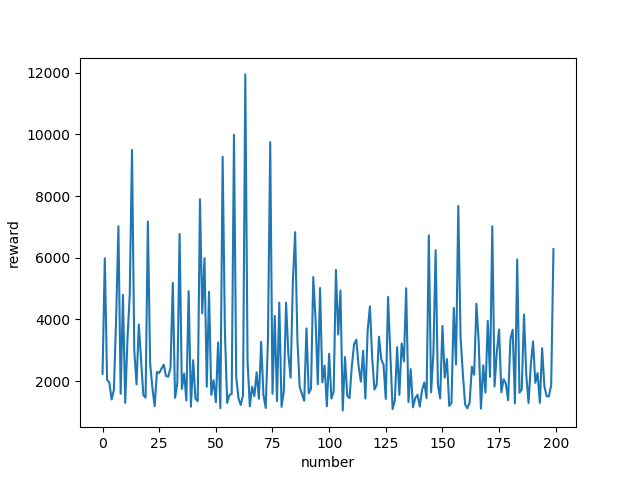
\includegraphics[height=8cm]{CartPole-1.png}
\caption{CartPole test-1}
\end{figure}

	MountainCar-v0任务中,我们获取的状态空间为[position,velocity]。我们设置边界值为它们原始的取值范围,将position分为5个箱,将velocity分为2个箱。设置轨迹最大长度为2000,最大训练轮数为2000,若连续100组训练的轨迹长度小于500就结束训练。对于训练得到的Q值表,进行了200测试,得到的奖赏和如图2所示。 
\begin{figure}[!h]
\centering
\small
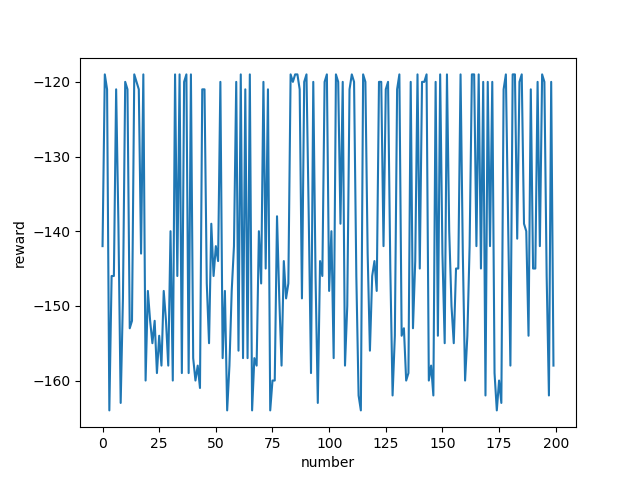
\includegraphics[height=8cm]{MountainCar-1.png}
\caption{MountainCar test-1}
\end{figure}

	Acrobot-v1任务中,我们获取的状态空间为[cos(theta1) sin(theta1) cos(theta2) sin(theta2) thetaDot1 thetaDot2],其中theta1为第一个关节与竖直方向的夹角,theta2为两个关节之间的夹角,thetaDot为对应角的角速度。在我的实验中只关注了两个角的角速度,忽略它的绝对位置。分别将thetaDot1和thetaDot2分为两个箱,边界值直接使用原始数据的取值范围。设置最长轨迹为2000,最大训练轮数为2000,若连续100组训练的轨迹长度小于150就结束训练。对于训练得到的Q值表,我们进行200组测试,得到的奖赏和如图3所示。
\begin{figure}[!h]
\centering
\small
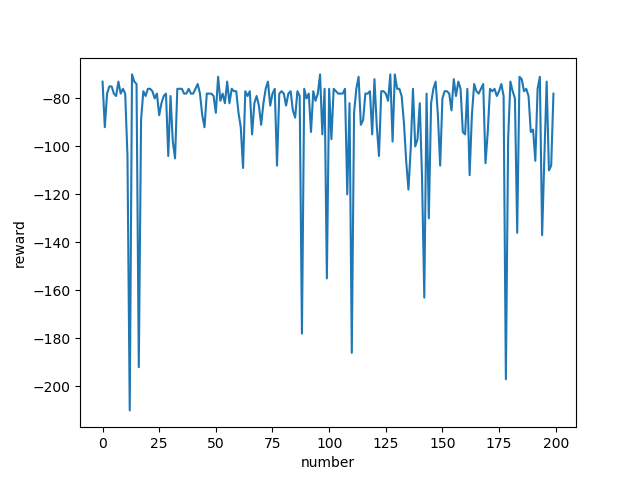
\includegraphics[height=8cm]{Acrobot-v1.png}
\caption{Acrobot test-1}
\end{figure}

	在Q-learning中我们希望在训练初期,Agent尽可能的进行“探索”并且较快的更新参数,在后期尽可能的进行“利用”并且较慢的更新参数。我们选择了两个指数下降的函数,$\epsilon = max(0.01,2(1-1/(1+math.exp(-i/30))$,$\alpha=max(0.1,min(0.5,1/(1+math.exp((i-30)/80))$,对应的函数图像如图4所示。最终Q-learning测试结果如表1所示。
\begin{figure}[!h]
\centering
\small
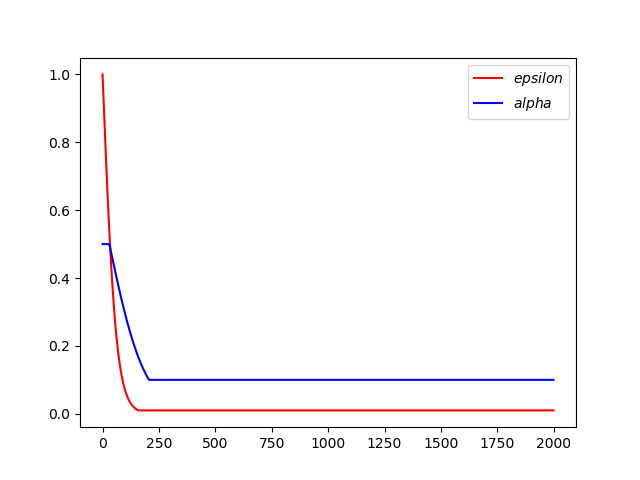
\includegraphics[height=8cm]{epsilon-alpha.png}
\caption{epsilon-alpha}
\end{figure}


\begin{table}[!h]
\caption{Q-learning训练结果}  
\centering
\begin{tabular*}{8cm}{lll}  
\hline  
Task & Mean 
 &  Standard deviation\\  
\hline  
CartPole-v0  & 2868.81 & 1915.78 \\  
Mountain-v0  & -139.83 & 16.43 \\ 
Acrobot-v1 	 & -86.82  & 22.19 \\ 
\hline  
\end{tabular*}  
\end{table} 

\section*{实验三. }
	\begin{algorithm}[!h]
	\renewcommand{\algorithmicrequire}{\textbf{Input:}}
	\renewcommand{\algorithmicensure}{\textbf{Output:}}
	\caption{Deep Q-learning with Experience Replay}
	\label{alg:2}
	\begin{algorithmic}[1]
		\STATE Initialize replay memory $D$ to capacity $N$
		\STATE Initialize action-value function $Q$ with random weights $\theta$
		\FOR{$episode=1$ to $M$}
			\FOR{$t=1$ to $T$}
			\STATE	$$a_t=
\begin{cases}
\text{Select from $A$ randomly \quad w.p.$\epsilon$}\\
\text{$max_a$$Q(s_t,a;\theta)$ \quad w.p.1-$\epsilon$ }
\end{cases}$$
\STATE Execute $a_t$ in emulator to observe reward $r_t$ and next state $s_{t+1}$
\STATE Store transition $(s_t,a_t,r_t,s_{t+1})$ in $D$
\STATE Sample random mini-batch of transitions $(s_j,a_j,r_j,s_{j+1})$ from $D$
\STATE	$$Set \quad y_j=
\begin{cases}
\text{$r_j$ \quad for terminal $s_{j+1}$}\\
\text{$r_j+\gamma max_{a'}Q(s_{t+1},a';\theta)$ for non-terminal $s_{j+1}$ }
\end{cases}$$
\STATE Update $\theta$ by gradient descent with loss function $(y_j-Q(s_j,a_j;\theta))^2$
			\ENDFOR
		\ENDFOR
\end{algorithmic}  
\end{algorithm}
	对于连续的状态-动作空间,另一种更为合理的方式是直接在连续的空间中进行学习。由于Q-learning需要穷举状态-动作对,所以面对连续状态-动作空间Q-learning无法适用。值函数近似Q-learning方法能够解决此类问题,若将值函数近似模型选取为一个深度网络,就是Deep Q-learning(DQN)算法。

	DQN算法伪代码如Algorithm 2所示。DQN算法基于Q-learning,算法框架和Q-learning完全相同,不同之处在于Q函数的表示和更新方式上。DQN中Q函数用一个深度网络表示,记为$Q(s,a;\theta)$,其中$a$表示状态,$a$表示执行的动作,$\theta$表示网络参数。DQN的目的是得到一个Q函数网络,对于一组状态动作对$(s,a)$,使得Q函数网络的输出$Q(s,a;\theta)$等于$(s,a)$下真实的Q值。具体到深度网络表示的Q函数模型上,Q函数的学习问题转化为了如何学习一组深度网络参数$\theta$使网络输出近似于真实的Q值。在本次实验中,我们只使用了一个隐层,设置隐层的节点数为64。

	CartPole-v0任务中,我们能够直接得到的reward只有1,直接使用效果比较差,所以我们根据观察值设置reward$=r_1+r_2$,其中$r_1=\frac{x_{threshold}-|x|}{x_{threshold}}-0.8$,$r_2=\frac{\theta_{threshold}-\theta}{\theta}-0.5$,$x$为杆子当前坐标,$x_{threshold}$表示杆子坐标的最大值,$\theta$表示杆子当前的倾斜角,$\theta_{threshold}$表示杆子最大倾斜角,所以$r_1$表示当前位置相对于原始位置的偏移程度,$r_2$表示当前杆子的倾斜程度。设置$M=500,T=20000,N=2000$,learning rate=0.0025,$\epsilon$为一个线性下降的函数,初始值为1,最终值为0.001,训练10000次后$\epsilon$降到最终值。在这个任务中,我们在Q函数网络中使用$sigmoid$函数作为激励函数。网络训练误差随训练轮数的变化关系如图5(a)所示,每轮训练之和随训练轮数的变化关系如图5(b)所示。在测试程序中,若连续训练5组的训练长度大于5000,就结束训练。我们对得到的Q函数网络进行200组测试,训练结果如图5(c)所示。

\begin{figure}[!h]
	\centering
	\subfigure[CartPole train loss]{
	  \centering
	 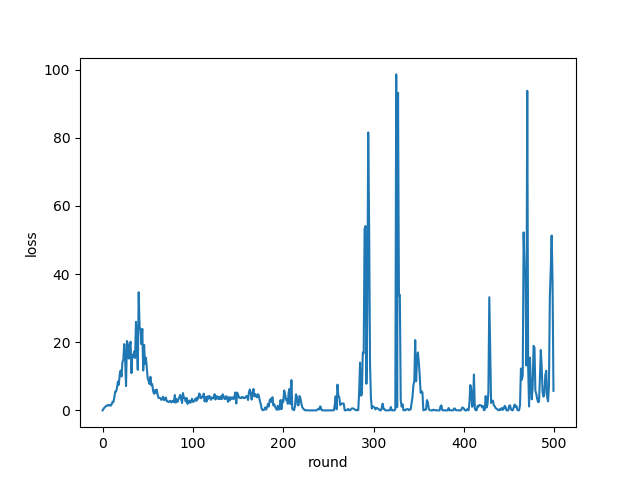
\includegraphics[width=4cm]{DQN-cartpole-loss.png}
	 }
	\subfigure[CartPole train reward]{
	  \centering
		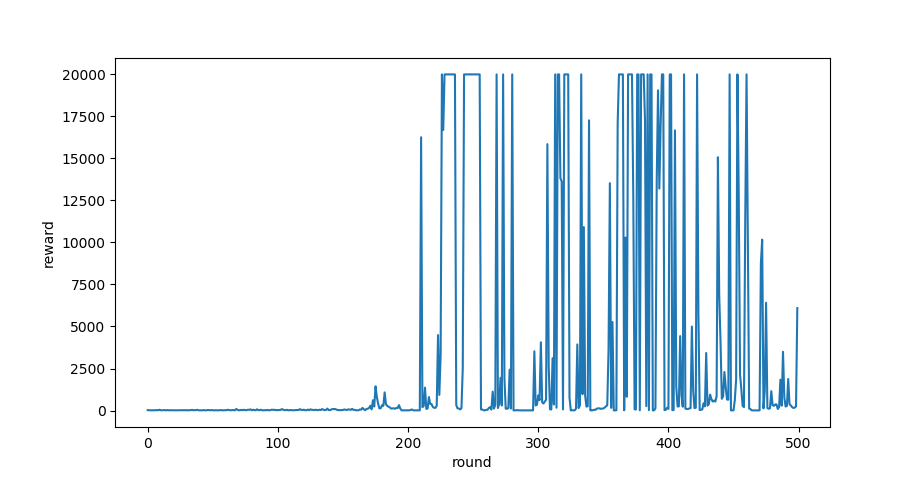
\includegraphics[width=4cm]{DQN-cartpole-distance.png}
	}
	\subfigure[CartPole test reward]{
	  \centering
		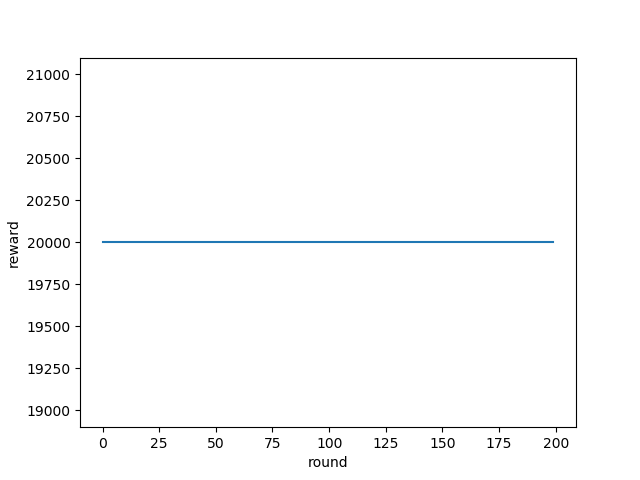
\includegraphics[width=4cm]{DQN-cartpole-result.png}
	}
	\caption{DQN CartPole-v0}

\end{figure}

	MountainCar-v0任务中,我们给done赋100的reward,设置$M=2000,T=2000,N=2000$,learning rate=0.005,$\epsilon$为一个线性下降的函数,初始值为1,最终值为0.01,训练10000次后$\epsilon$降到最终值,激励函数为$relu$。网络训练误差随训练轮数的变化关系如图6(a)所示,每轮训练之和随训练轮数的变化关系如图6(b)所示。在测试程序中,若连续训练100组的训练长度小于500,就结束训练。我们对得到的Q函数网络进行200组测试,训练结果如图6(c)所示。


\begin{figure}[!h]
	\centering
	\subfigure[MountainCar train loss]{
	  \centering
	 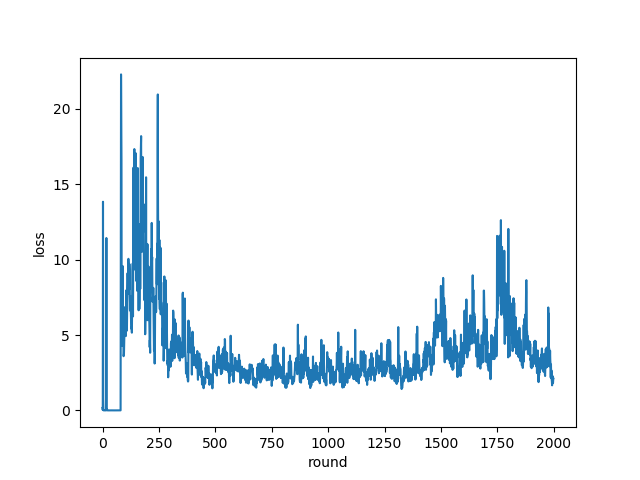
\includegraphics[width=4cm]{DQN-mountain-loss.png}
	 }
	\subfigure[MountainCar train reward]{
	  \centering
		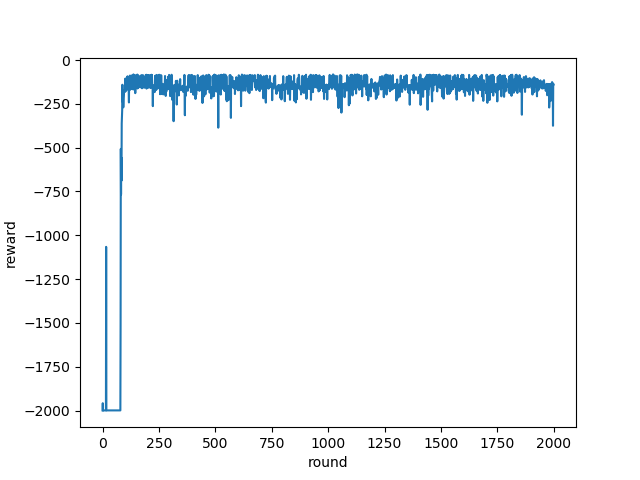
\includegraphics[width=4cm]{DQN-mountain-distance.png}
	}
	\subfigure[MountainCar test reward]{
	  \centering
		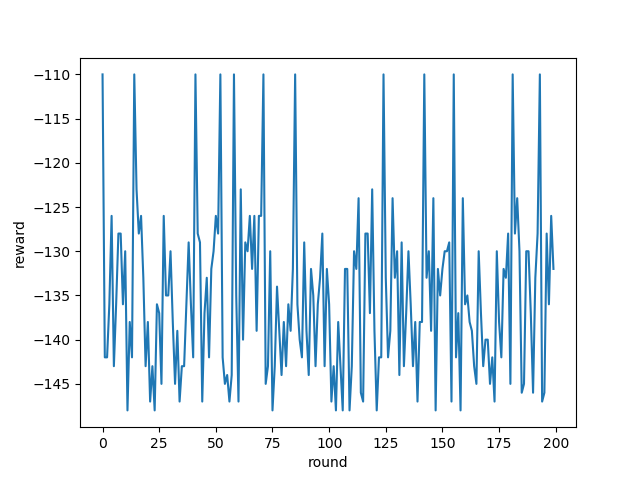
\includegraphics[width=4cm]{DQN-mountain-result.png}
	}
	\caption{DQN MountainCar-v0}

\end{figure}

	Acrobot-v1任务中,我们给done赋100的reward,设置$M=2000,T=2000,N=2000$,learning rate=0.005,$\epsilon$为一个线性下降的函数,初始值为1,最终值为0.1,训练10000次后$\epsilon$降到最终值,激励函数为$relu$。网络训练误差随训练轮数的变化关系如图7(a)所示,每轮训练之和随训练轮数的变化关系如图7(b)所示。在测试程序中,若连续训练100组的训练长度小于500,就结束训练。我们对得到的Q函数网络进行200组测试,训练结果如图7(c)所示。三个任务DQN的测试统计量如表2所示。


\begin{figure}[!h]
	\centering
	\subfigure[Acrobot train loss]{
	  \centering
	 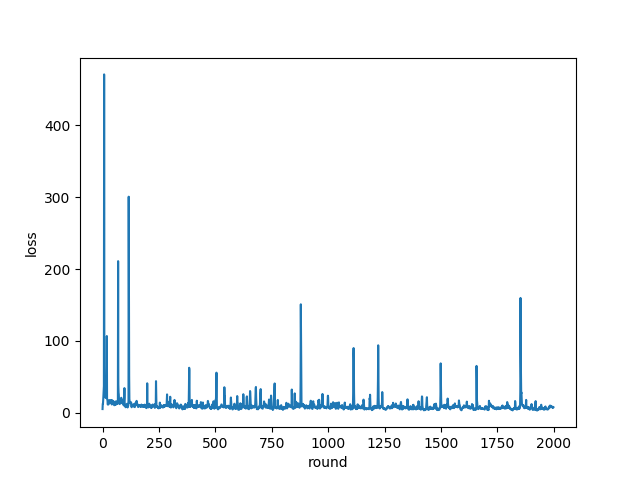
\includegraphics[width=4cm]{DQN-acrobot-loss.png}
	 }
	\subfigure[Acrobot train reward]{
	  \centering
		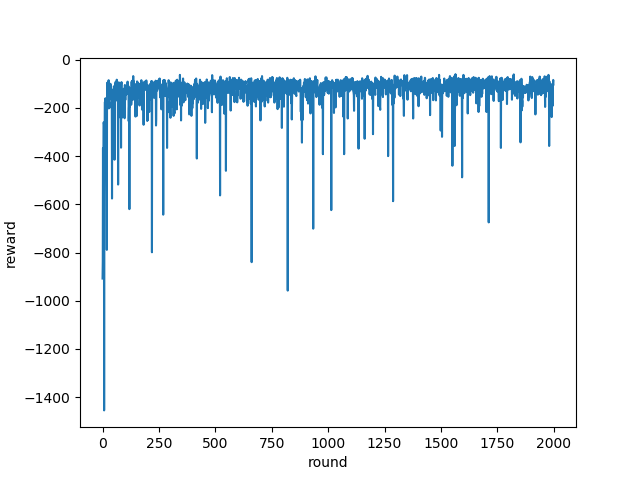
\includegraphics[width=4cm]{DQN-acrobot-distance.png}
	}
	\subfigure[Acrobot test reward]{
	  \centering
		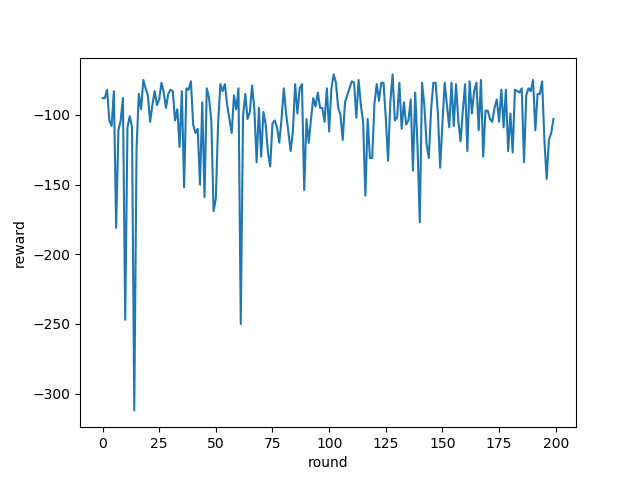
\includegraphics[width=4cm]{DQN-acrobot-result.png}
	}
	\caption{DQN Acrobot-v0}

\end{figure}


\begin{table}[!h]
\caption{DQN训练结果}  
\centering
\begin{tabular*}{8cm}{lll}  
\hline  
Task & Mean 
 &  Standard deviation\\  
\hline  
CartPole-v0  & 20000 & 0 \\  
Mountain-v0  & -127.44 & 31.43 \\ 
Acrobot-v1 	 & -102.82  & 28.19 \\ 
\hline  
\end{tabular*}  
\end{table} 

	

	
\section*{实验四. }
	\begin{algorithm}[!h]
	\renewcommand{\algorithmicrequire}{\textbf{Input:}}
	\renewcommand{\algorithmicensure}{\textbf{Output:}}
	\caption{Improved Deep Q-learning with Experience Replay}
	\label{alg:3}
	\begin{algorithmic}[1]
		\STATE Initialize replay memory $D$ to capacity $N$
		\STATE Initialize action-value function $Q$ with random weights $\theta$
		\STATE target action-value function $\hat{Q}$ with weight $\theta^-=\theta$
		\FOR{$episode=1$ to $M$}
			\FOR{$t=1$ to $T$}
			\STATE	$$a_t=
\begin{cases}
\text{Select from $A$ randomly \quad w.p.$\epsilon$}\\
\text{$max_a$$Q(s_t,a;\theta)$ \quad w.p.1-$\epsilon$ }
\end{cases}$$
\STATE Execute $a_t$ in emulator to observe reward $r_t$ and next state $s_{t+1}$
\STATE Store transition $(s_t,a_t,r_t,s_{t+1})$ in $D$
\STATE Sample random mini-batch of transitions $(s_j,a_j,r_j,s_{j+1})$ from $D$
\STATE	$$Set \quad y_j=
\begin{cases}
\text{$r_j$ \quad for terminal $s_{j+1}$}\\
\text{$r_j+\gamma max_{a'}\hat{Q}(s_{t+1},a';\theta)$ for non-terminal $s_{j+1}$ }
\end{cases}$$
\STATE Update $\theta$ by gradient descent with loss function $(y_j-Q(s_j,a_j;\theta))^2$
\STATE Every $C$ steps reset $\hat{Q}=Q$
			\ENDFOR
		\ENDFOR
\end{algorithmic}  
\end{algorithm}

	在DQN中,每在任务环境中探索一步均要更新一次网络权重。这样的更新方式是不稳定的,对学习Q值网络不利。改进版本的DQN如Algorithm 3所示,在原始DQN上增加了一个Target Q网络。原始DQN的目标Q网络是动态变化的,随着Q网络的更新而变化,这导致了目标Q值和当前Q值相关性较大。Improved DQN增加了一个单独的目标Q网络,每隔一段时间将Q网络的参数赋给Target Q,以提高系统的稳定性。

	在本次实验中,我们使用和实验三相同的reward和$\epsilon$贪心策略。在CartPole-v0中,我们设置$M=500,T=20000,N=2000$,最小$\epsilon=0.001$,更新步长$C=100$,网络训练误差随训练轮数的变化关系如图8(a)所示,每轮训练之和随训练轮数的变化关系如图8(b)所示。在测试程序中,若连续20组训练的长度超过10000,就停止训练。我们对得到的Q函数网络进行200组测试,训练结果如图8(c)所示。

\begin{figure}[!h]
	\centering
	\subfigure[CartPole train loss]{
	  \centering
	 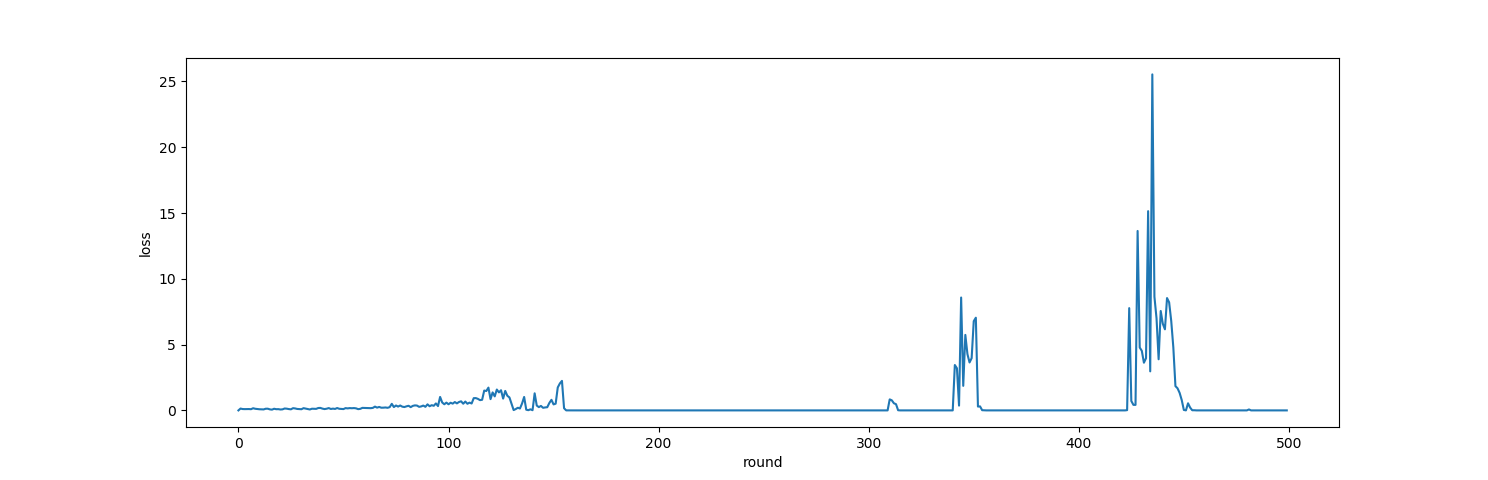
\includegraphics[width=4cm]{ImprovedDQN-cartpole-loss.png}
	 }
	\subfigure[CartPole train reward]{
	  \centering
		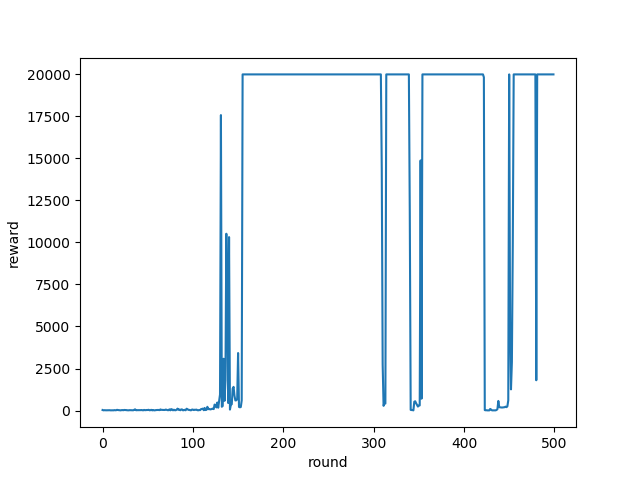
\includegraphics[width=4cm]{ImprovedDQN-cartpole-distance.png}
	}
	\subfigure[CartPole test reward]{
	  \centering
		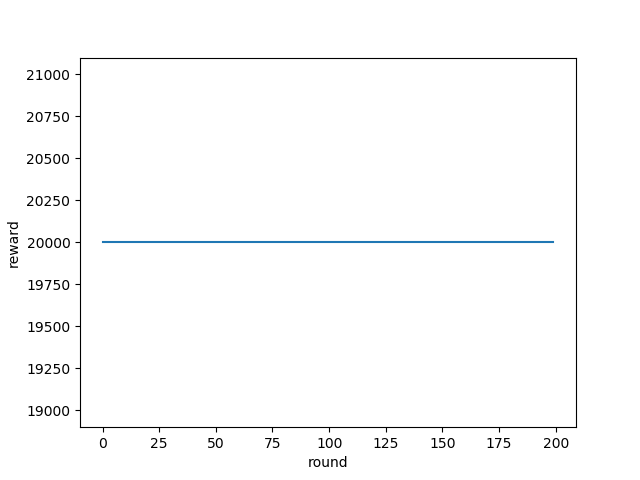
\includegraphics[width=4cm]{DQN-cartpole-result.png}
	}
	\caption{ImprovedDQN CartPole-v0}

\end{figure}

	在MountainCar-v0中,我们设置$M=2000,T=2000,N=2000$,最小$\epsilon=0.01$,更新步长$C=100$,网络训练误差随训练轮数的变化关系如图9(a)所示,每轮训练之和随训练轮数的变化关系如图9(b)所示。在测试程序中,若连续100组训练的长度小于500,就停止训练。我们对得到的Q函数网络进行200组测试,训练结果如图9(c)所示。

\begin{figure}[!h]
	\centering
	\subfigure[MountainCar train loss]{
	  \centering
	 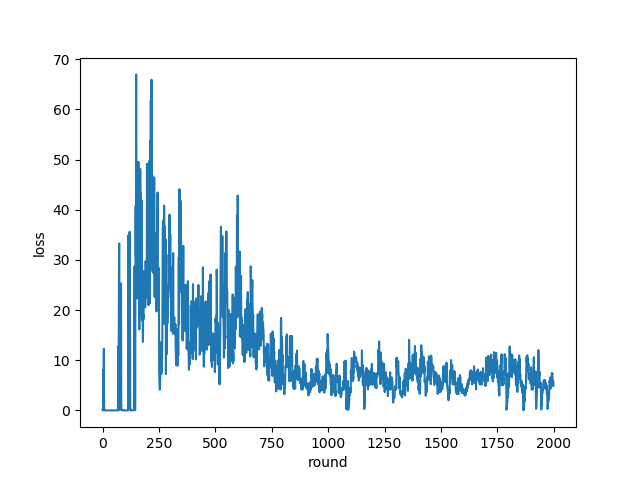
\includegraphics[width=4cm]{ImprovedDQN-mountain-loss.png}
	 }
	\subfigure[MountainCar train reward]{
	  \centering
		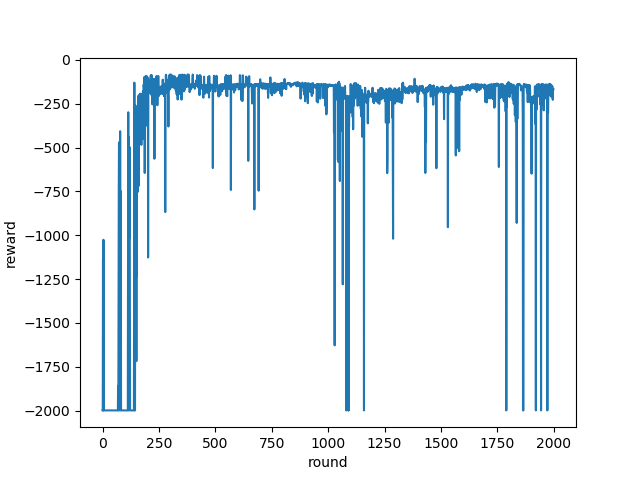
\includegraphics[width=4cm]{ImprovedDQN-mountain-distance.png}
	}
	\subfigure[MountainCar test reward]{
	  \centering
		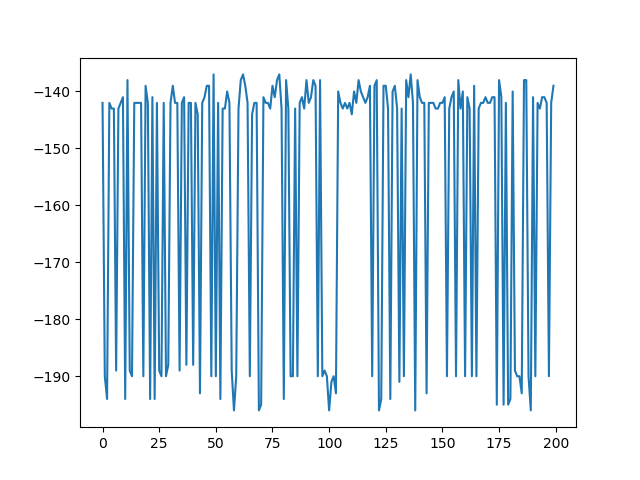
\includegraphics[width=4cm]{ImprovedDQN-mountain-result.png}
	}
	\caption{ImprovedDQN MountainCar-v0}

\end{figure}

	在Acrobot-v0中,我们设置$M=2000,T=2000,N=2000$,最小$\epsilon=0.01$,更新步长$C=100$,网络训练误差随训练轮数的变化关系如图10(a)所示,每轮训练之和随训练轮数的变化关系如图10(b)所示。在测试程序中,若连续100组训练的长度小于300,就停止训练。我们对得到的Q函数网络进行200组测试,训练结果如图10(c)所示。三个任务ImprovedDQN的测试统计量如表3所示。


\begin{figure}[!h]
	\centering
	\subfigure[Acrobot train loss]{
	  \centering
	 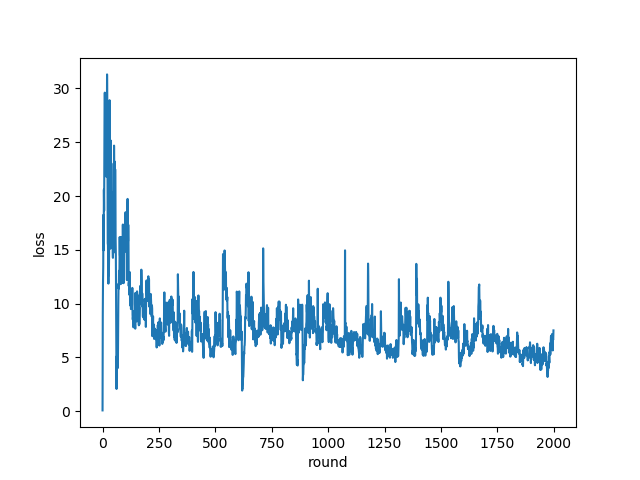
\includegraphics[width=4cm]{ImprovedDQN-acrobot-loss.png}
	 }
	\subfigure[Acrobot train reward]{
	  \centering
		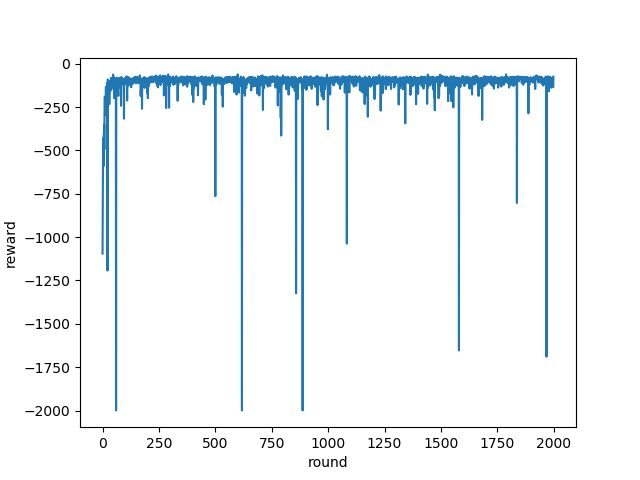
\includegraphics[width=4cm]{ImprovedDQN-acrobot-distance.png}
	}
	\subfigure[Acrobot test reward]{
	  \centering
		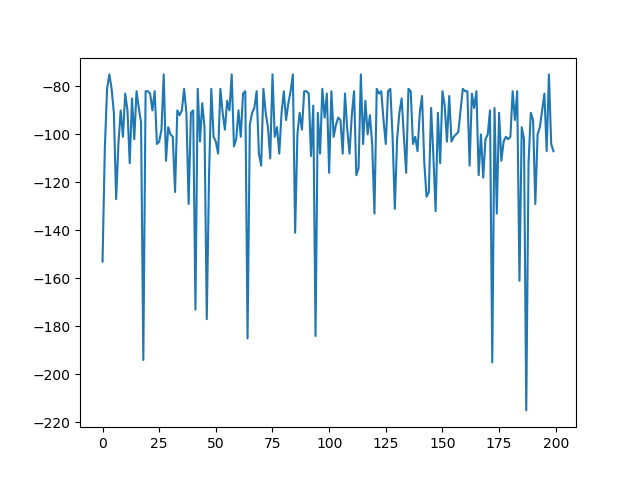
\includegraphics[width=4cm]{ImprovedDQN-acrobot-result.png}
	}
	\caption{ImprovedDQN Acrobot-v0}

\end{figure}


\begin{table}[!h]
\caption{ImprovedDQN训练结果}  
\centering
\begin{tabular*}{8cm}{lll}  
\hline  
Task & Mean 
 &  Standard deviation\\  
\hline  
CartPole-v0  & 20000 & 0 \\  
Mountain-v0  & -156.59 & 23.43 \\ 
Acrobot-v1 	 & -97.90  & 22.76 \\ 
\hline  
\end{tabular*}  
\end{table} 




\end{document}